% introduction

% example: flow velocity imaging
\begin{frame}{Example: flow imaging}
	\begin{figure}
		\centering
		\includegraphics [width=0.8\textwidth, trim=5 5 5 5, clip] {%
			c,intro/flow%
		}%
	\end{figure}
	\vspace{-0.5cm}
	\makebox[4.2cm][r]{qualitative}
	\makebox[4.2cm][r]{%
		quantitative
		\footnote{%
			figure borrowed from \citec{hope:13:cao}%
		}%
	}%
	\vspace{0.3cm}
\end{frame}

% example: diffusion imaging
\begin{frame}{Example: diffusion imaging}
	\begin{figure}
		\centering
		\includegraphics [width=\textwidth] {%
			c,intro/dti%
		}%
	\end{figure}
	\vspace{-0.5cm}
	\makebox[2.5cm][r]{qualitative}
	\makebox[4.8cm][r]{fractional anisotropy (FA)}
	\makebox[2.7cm][r]{%
		directional FA
		\footnote{%
			figure borrowed from \href{%
				http://www.diffusion-imaging.com/2009/05/diffusion-tensor-imaging-101.html
			}{%
				\textcolor{arch-ivy}{www.diffusion-imaging.com}
			}%
		}%
	}%
\end{frame}

% example: myelin water imaging
\begin{frame}{Example: myelin water imaging}
	\vspace{-1cm}
	\begin{figure}
		\centering
		\begin{minipage}[b]{0.48\textwidth}
			\centering
			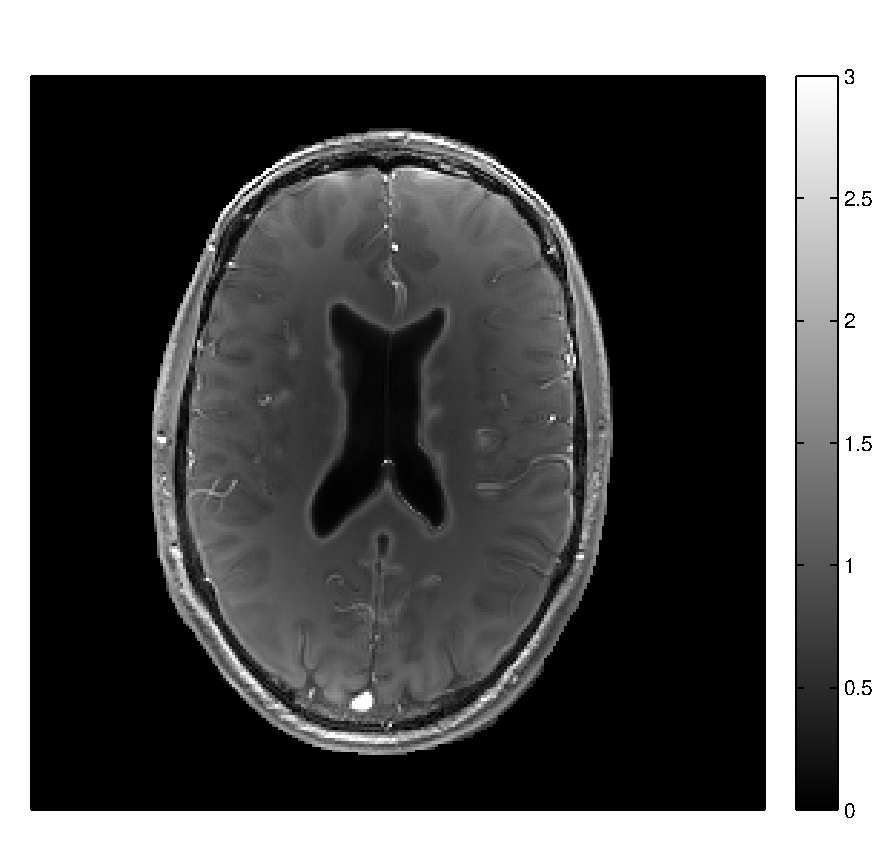
\includegraphics [height=5cm, trim={0 0 50 0}, clip] {%
				c,intro/mwi-roi.eps%
			}%
		\end{minipage}
		\begin{minipage}[b]{0.48\textwidth}
			\centering
			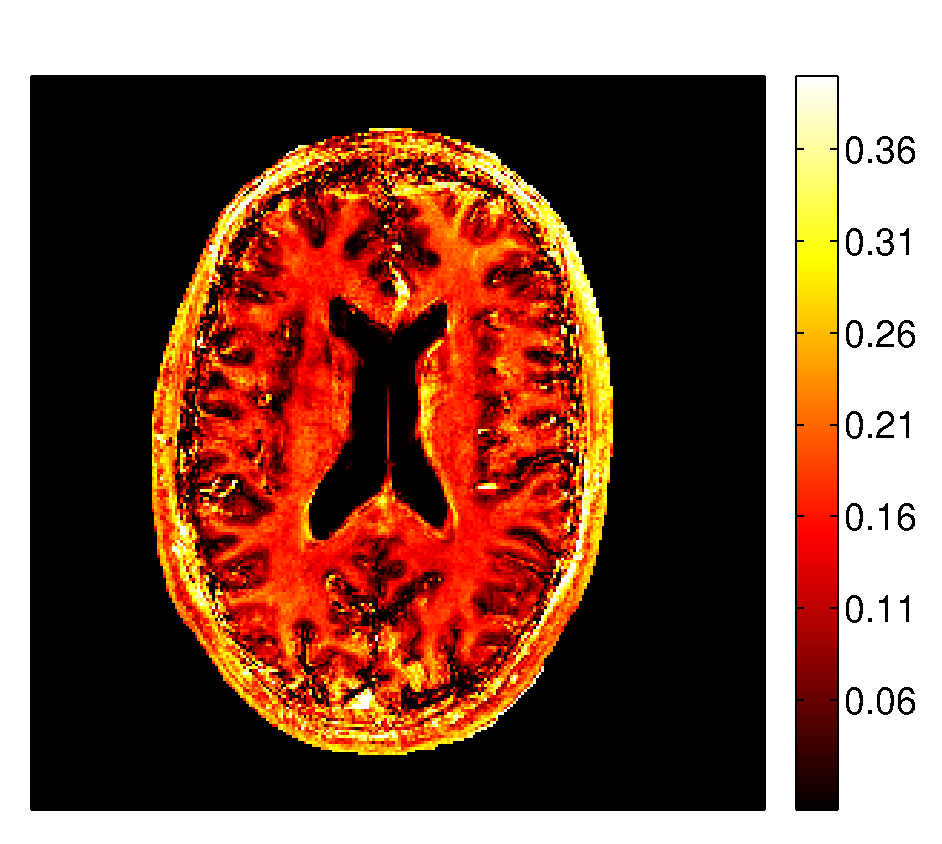
\includegraphics [height=5cm] {%
				c,intro/mwi-ff.eps%
			}%
		\end{minipage}
	\end{figure}
	\vspace{-0.5cm}
	\makebox[3.6cm][r]{qualitative}
	\makebox[6cm][r]{%
		fast-relaxing fraction
		\footnote{%
			figure adapted from \citec{nataraj:17:mwf}
		}%
	}%
\end{frame}

% intro
\begin{frame}{Quantitative MRI (QMRI)}
	\uncover<1->{
		\textbf{Goal}: 
		\hlb{rapidly} and \hlg{accurately} \hlo{localize} \hlm{biomarkers} from MR data
	}
	\begin{itemize}
		\item<2>{
			\makebox[1.8cm][l]{\hlm{biomarker}} measurable tissue property (\eg, flow rate) \\
			\makebox[1.8cm][l]{} that indicates a biological process (\eg, blockage) \\
			\makebox[1.8cm][l]{} characteristic to specific disorders (\eg, stroke)
		}
		\item<3>{\makebox[1.8cm][l]{\hlo{localize}} produce quantitative MR images}
		\item<4>{\makebox[1.8cm][l]{\hlg{accurately}} physically realistic signal models}
		\item<4>{\makebox[1.8cm][l]{\hlb{rapidly}} fast acquisition, fast estimation}
	\end{itemize}
	
	\uncover<5->{
		\textbf{Challenge:} \hlb{rapidly} vs. \hlg{accurately} often competing goals
		\begin{itemize}
			\item{more accurate models typically depend on more markers}
			\item{precisely estimating more markers usually requires \\ longer scans and more computation}
		\end{itemize}
	}
\end{frame}